\documentclass[final]{beamer}
\usepackage[orientation=landscape, width=36",height=24", scale=.8]{beamerposter}
\usepackage{graphicx}	
\usepackage{adjustbox}
\usepackage{caption}
\usepackage{pbox}
\usepackage{ragged2e} 
\usepackage{booktabs} % Top and bottom rules for tables

\usetheme{confposter}
\usepackage{exscale}
\usepackage{graphicx}  % Required for including images
\graphicspath{ {../images/} }


\usepackage {tikz}
\usetikzlibrary{arrows}
\usetikzlibrary{shapes.misc, positioning, shapes.geometric}

\newlength{\sepwid}
\newlength{\onecolwid}
\newlength{\twocolwid}
\newlength{\threecolwid}
%\setlength{\paperwidth}{48in} % A0 width: 46.8in
%\setlength{\paperheight}{36in} % A0 height: 33.1in
\setlength{\sepwid}{0.007\paperwidth} % Separation width (white space) between columns
\setlength{\onecolwid}{0.324\paperwidth} % Width of one column
\setlength{\twocolwid}{0.464\paperwidth} % Width of two columns
\setlength{\threecolwid}{0.708\paperwidth} % Width of three columns
\setlength{\topmargin}{-0.5in} % Reduce the top margin size

\setbeamercolor{block title}{fg=Maroon,bg=white} %
%\usetheme{Frankfurt}
%\usecolortheme{beetle}
%\setbeamercolor{block body}{fg=black,bg=white} % Colors of the body of blocks
%\setbeamertemplate{navigation symbols}{}%remove navigation symbols
%\setbeamertemplate{footline}[frame number]{}

\usecaptiontemplate{
	\small\structure{\insertcaptionname~\insertcaptionnumber:}
	\insertcaption}


\begin{document}
	
\begin{frame}[t, noframenumbering,plain]{}

\begin{block}{\centering \Huge {An Novel RNN Approach to Classification of Complex Textual Scientific Metadata}}
	\begin{center}
		\Large{
			Reid McIlroy-Young\quad MACS 302 Final Poster \quad June 1, 2017}
	\end{center}
\end{block}


\begin{columns}[t] 
	
	%\begin{column}{\sepwid}\end{column} 
	\begin{column}{\onecolwid} 

		\begin{alertblock}{Introduction}
			\justifying
			Currently most analysis of scientific publications is limited to those fields available in the database used by the researchers. Efforts to extend the fields usually rely on unsupervised clustering (e.g. Boyack, \textit{et al}, 2005). Presented here is a new technique for using supervised classification on scientific metadata, with imperfect training data. By using a complex model that is reading the unstructured text we can define much more abstract concepts than a similarity measure. For this analysis we looked for \textit{papers introducing new software packages, tools or interfaces}. 
		\end{alertblock}
		\begin{alertblock}{Data}
			\justifying
			Our data are all articles published in the top 123 statistics journals, as identified by the Web of Science (WOS), between 2005 and 2015, giving a total of 78 971 articles. The data were provided by the WOS mirror database hosted by Knowledge Lab. From these, three journals were identified that primarily introduce new software and eight that almost never do so. These gave us 1251 positive examples and 4362 negative for training. Because we are using journal names alone and no hand coding some small fraction of our training data is incorrectly labelled.
		\end{alertblock}

	
	\begin{alertblock}{Computation Graph}
		\justifying
		The neural network (NN) can be understood as a computation graph with the weights being computed via backpropagation through the graph. Figure \ref{rnn} shows the partiality unfolded graph, with the circular nodes being those learned in training. 
	\end{alertblock}
	\begin{block}{}
		\begin{figure}[!ht]
			\centering
			
			\begin{tikzpicture}[shorten >=1pt,auto,node distance=4cm, very thick]
			\node[draw, rounded corners] (1) {Abstract};
			\node[draw, rounded corners] (tokenizer) [above = 1cm of 1] {Tokenizer};
			\node[draw, rounded corners] (2) [above = 1cm of tokenizer] {word2vec};
			\node[draw] (3) [above of=2] {$\vec{x}_{t}$};
			\node[draw] (4) [left of =3] {$\vec{x}_{t-1}$};
			\node[draw] (5) [right of =3] {$\vec{x}_{t+1}$};
			
			\node[draw, circle] (h1) [above of=3] {$h_t^1$};
			\node[draw, circle] (h2) [above of=4] {$h_{t-1}^1$};
			\node[draw, circle] (h3) [above of=5] {$h_{t+1}^1$};
			
			\node[draw, circle] (g1) [above of=h1] {$g_t^1$};
			\node[draw, circle] (g2) [above of=h2] {$g_{t-1}^1$};
			\node[draw, circle] (g3) [above of=h3] {$g_{t+1}^1$};
			
			\node[draw, circle] (h12) [above of=g1] {$h_t^2$};
			\node[draw, circle] (h22) [above of=g2] {$h_{t-1}^2$};
			\node[draw, circle] (h32) [above of=g3] {$h_{t+1}^2$};
			
			\node[draw, circle] (g12) [above of=h12] {$g_t^2$};
			\node[draw, circle] (g22) [above of=h22] {$g_{t-1}^2$};
			\node[draw, circle] (g32) [above of=h32] {$g_{t+1}^2$};
			
			\node[draw, regular polygon, regular polygon sides=6] (L) [above of=g12] {$\oplus$};
			
			\node[draw, rounded corners] (1t) [right = 10cm of 1]{Title};
			\node[draw, rounded corners] (tokenizert) [above = 1cm of 1t] {Tokenizer};
			\node[draw, rounded corners] (2t) [above = 1cm of tokenizert] {word2vec};
			
			\node[draw] (3t) [above of=2t] {$\vec{x}_{t}$};
			\node[draw] (4t) [left of =3t] {$\vec{x}_{t-1}$};
			\node[draw] (5t) [right of =3t] {$\vec{x}_{t+1}$};
			
			\node[draw, circle] (h1t) [above of=3t] {$h^{ t}_1$};
			\node[draw, circle] (h2t) [above of=4t] {$h^{ t-1}_1$};
			\node[draw, circle] (h3t) [above of=5t] {$h^{t+1}_1$};
			
			\node[draw, circle] (g1t) [above of=h1t] {$g^{t}_1$};
			\node[draw, circle] (g2t) [above of=h2t] {$g^{t-1}_1$};
			\node[draw, circle] (g3t) [above of=h3t] {$g^{t+1}_1$};
			
			\node[draw, circle] (h1t2) [above of=g1t] {$h^{ t}_2$};
			\node[draw, circle] (h2t2) [above of=g2t] {$h^{ t-1}_2$};
			\node[draw, circle] (h3t2) [above of=g3t] {$h^{t+1}_2$};
			
			\node[draw, circle] (g1t2) [above of=h1t2] {$g^{t}_2$};
			\node[draw, circle] (g2t2) [above of=h2t2] {$g^{t-1}_2$};
			\node[draw, circle] (g3t2) [above of=h3t2] {$g^{t+1}_2$};
			
			
			\node[draw, regular polygon, regular polygon sides=6] (Lt) [above of=g1t2] {$\oplus$};
			\node[draw, circle] (u) [above right = 7.2cm of L]{$u$};
			\node[draw] (y) [above of = u]{$\hat{y}$};
			
			
			\draw[->] (L) -- (u);
			\draw[->] (Lt) -- (u);
			\draw[->] (u) -- (y);
			
			\draw[->] (1) -- (tokenizer);
			\draw[->] (tokenizer) -- (2);
			\draw[->] (2) -- (3);
			\draw[->] (2) -- (4);
			\draw[->] (2) -- (5);
			
			\draw[->] (3) -- (h1);
			\draw[->] (4) -- (h2);
			\draw[->] (5) -- (h3);
			\draw[->] (h2) -- (h1);
			\draw[->] (h1) -- (h3);
			
			\draw[->] (3)  edge[bend left] (g1);
			\draw[->] (4) edge[bend left] (g2);
			\draw[->] (5) edge[bend left] (g3);
			\draw[->] (g1) -- (g2);
			\draw[->] (g3) -- (g1);
			
			\draw[->] (h1)  edge[bend left] (h12);
			\draw[->] (h2) edge[bend left] (h22);
			\draw[->] (h3) edge[bend left] (h32);
			\draw[->] (h22) -- (h12);
			\draw[->] (h12) -- (h32);
			
			\draw[->] (g1)  edge[bend right] (g12);
			\draw[->] (g2) edge[bend right] (g22);
			\draw[->] (g3) edge[bend right] (g32);
			\draw[->] (g12) -- (g22);
			\draw[->] (g32) -- (g12);
			
			\draw[->] (g22) -- (L);
			\draw[->] (h32) -- (L);
			
			\draw[->] (1t) -- (tokenizert);
			\draw[->] (tokenizert) -- (2t);
			\draw[->] (2t) -- (3t);
			\draw[->] (2t) -- (4t);
			\draw[->] (2t) -- (5t);
			
			\draw[->] (3t) edge[bend right] (h1t);
			\draw[->] (4t) edge[bend right] (h2t);
			\draw[->] (5t) edge[bend right] (h3t);
			\draw[->] (h2t) -- (h1t);
			\draw[->] (h1t) -- (h3t);
			
			\draw[->] (3t)  edge[bend left] (g1t);
			\draw[->] (4t) edge[bend left] (g2t);
			\draw[->] (5t) edge[bend left] (g3t);
			\draw[->] (g1t) -- (g2t);
			\draw[->] (g3t) -- (g1t);
			
			\draw[->] (h1t)  edge[bend left] (h1t2);
			\draw[->] (h2t) edge[bend left] (h2t2);
			\draw[->] (h3t) edge[bend left] (h3t2);
			\draw[->] (h2t2) -- (h1t2);
			\draw[->] (h1t2) -- (h3t2);
			
			\draw[->] (g1t)  edge[bend right] (g1t2);
			\draw[->] (g2t) edge[bend right] (g2t2);
			\draw[->] (g3t) edge[bend right] (g3t2);
			\draw[->] (g1t2) -- (g2t2);
			\draw[->] (g3t2) -- (g1t2);
			
			\draw[->] (g2t2) -- (Lt);
			\draw[->] (h3t2) -- (Lt);
			\end{tikzpicture}
			\caption{Simplified recursive bidirectional Recursive NN (RNN) layout, LSTM connections were removed for clarity. Circles are NN layers, rectangles with curved corners are the preprocessing, hexagons are combined outputs from the RNN layers, and final output and inputs are indicated with squared corners.}\label{rnn}
		\end{figure}
	\end{block}

	\end{column} 

%\begin{column}{\sepwid}\end{column} % Empty spacer column

\begin{column}{\onecolwid} % Begin a column which is two columns wide (column 2)
	\begin{alertblock}{Methods}
		\justifying
		For our analysis we have two pieces of text for each article that we provide to the model, the abstract and title; since from these most humans can quickly identify if the article describes a new piece of software. Note these fields are both unstructured text with some even being non-English. To convert these into usable form we first tokenize them at the word and sentence levels, then trained a 200-dimensional Word2Vec embedding model from all tokens in the data set. Note that, no tokens are dropped at any point, the Word2Vec model is trained with both punctuation and highly infrequent tokens.
		
		Our classifier is a Recursive NN composed of two parallel bidirectional two-layer recurrent NNs (RNNs) using Long Short-Term Memory (LSTM) cells whose outputs are provided to a final single fully connected layer. Both input layers have $200$ nodes, the hidden RNN layers are all $256$ nodes and the final output is $2$ nodes. The inputs to each of our RNNs are sequences of Word2Vec vectors for each of the word level tokens, sentence levels are ignored but all punctuation has a Word2Vec vector so the RNN can learn to recognize sentences.
		
		To train the model the weights were updated with automatic backpropagation against the cross entropy loss. Since the positives are greatly outnumber by the negatives we added them twice to the training set, so there was a $36.8\%$ chance of a positive example being chosen for a batch. $10\%$ of the testing set was held out for cross-validation and the final results are shown in Table \ref{t1}.
		
		\begin{table}
			\vspace{2ex}
			\begin{tabular}{l r}
				\toprule
				Epochs & 8  \\
				Batches per Epoch & 500\\
				Testing Loss &   0.093 \\
				Testing Error Rate & 0.023 \\
				Detection Rate & 0.955\\
				False Positive Rate& 0.017\\
				\bottomrule
			\end{tabular}
			\caption{Testing results for optimal model}\label{t1}
		\end{table}
	\end{alertblock}
	\begin{alertblock}{RNN Layers}
		\justifying
		Getting a model that can make classifications with a $4\%$ error rate is very good, but we want to know if the model has some understanding of its inputs or if it is simply looking for words (e.g. `\textit{R}') or sequences of words (e.g. `\textit{a new package}'). To do this we can look at the outputs from the RNN layers to the fully connected layer $u$, these are updated for each word and only the final values are provided to the hidden layer, specificity we are seeing  the outputs from $g^2$ and $h^2$ in figure \ref{rnn} concatenated into a $512$ dimensional vector. Figures \ref{title} and \ref{abstract} show the activations for each word in the title and abstract respectively, of a positive and negative sample. We can see by examining these plots that both RNNs have somewhat nuanced understandings of their inputs.
	\end{alertblock}
	\vspace{1cm}
\begin{columns}[t,totalwidth=\onecolwid] % Split up the two columns wide column
	
	\begin{column}{.49\onecolwid}\vspace{-.6in} % The first column within column 2 (column 2.1)

		\begin{block}
			
			\begin{figure}
				\centering
				\begin{adjustbox}{center}
				\includegraphics[width=0.55\onecolwid]{comparisonTitle.pdf}
				\end{adjustbox}
				\caption[skip=20pt]{RNN activations for each word in two titles; the positive example is on top, the negative below it, and a comparison of each input's final output is shown at the bottom.}\label{title}
				
			\end{figure}
			
		\end{block}
		
	\end{column} % End of column 2.1
	
	\begin{column}{.49\onecolwid}\vspace{-.6in} % The second column within column 2 (column 2.2)
		\begin{block}{}
			\begin{figure}
				\centering
				\begin{adjustbox}{center}
				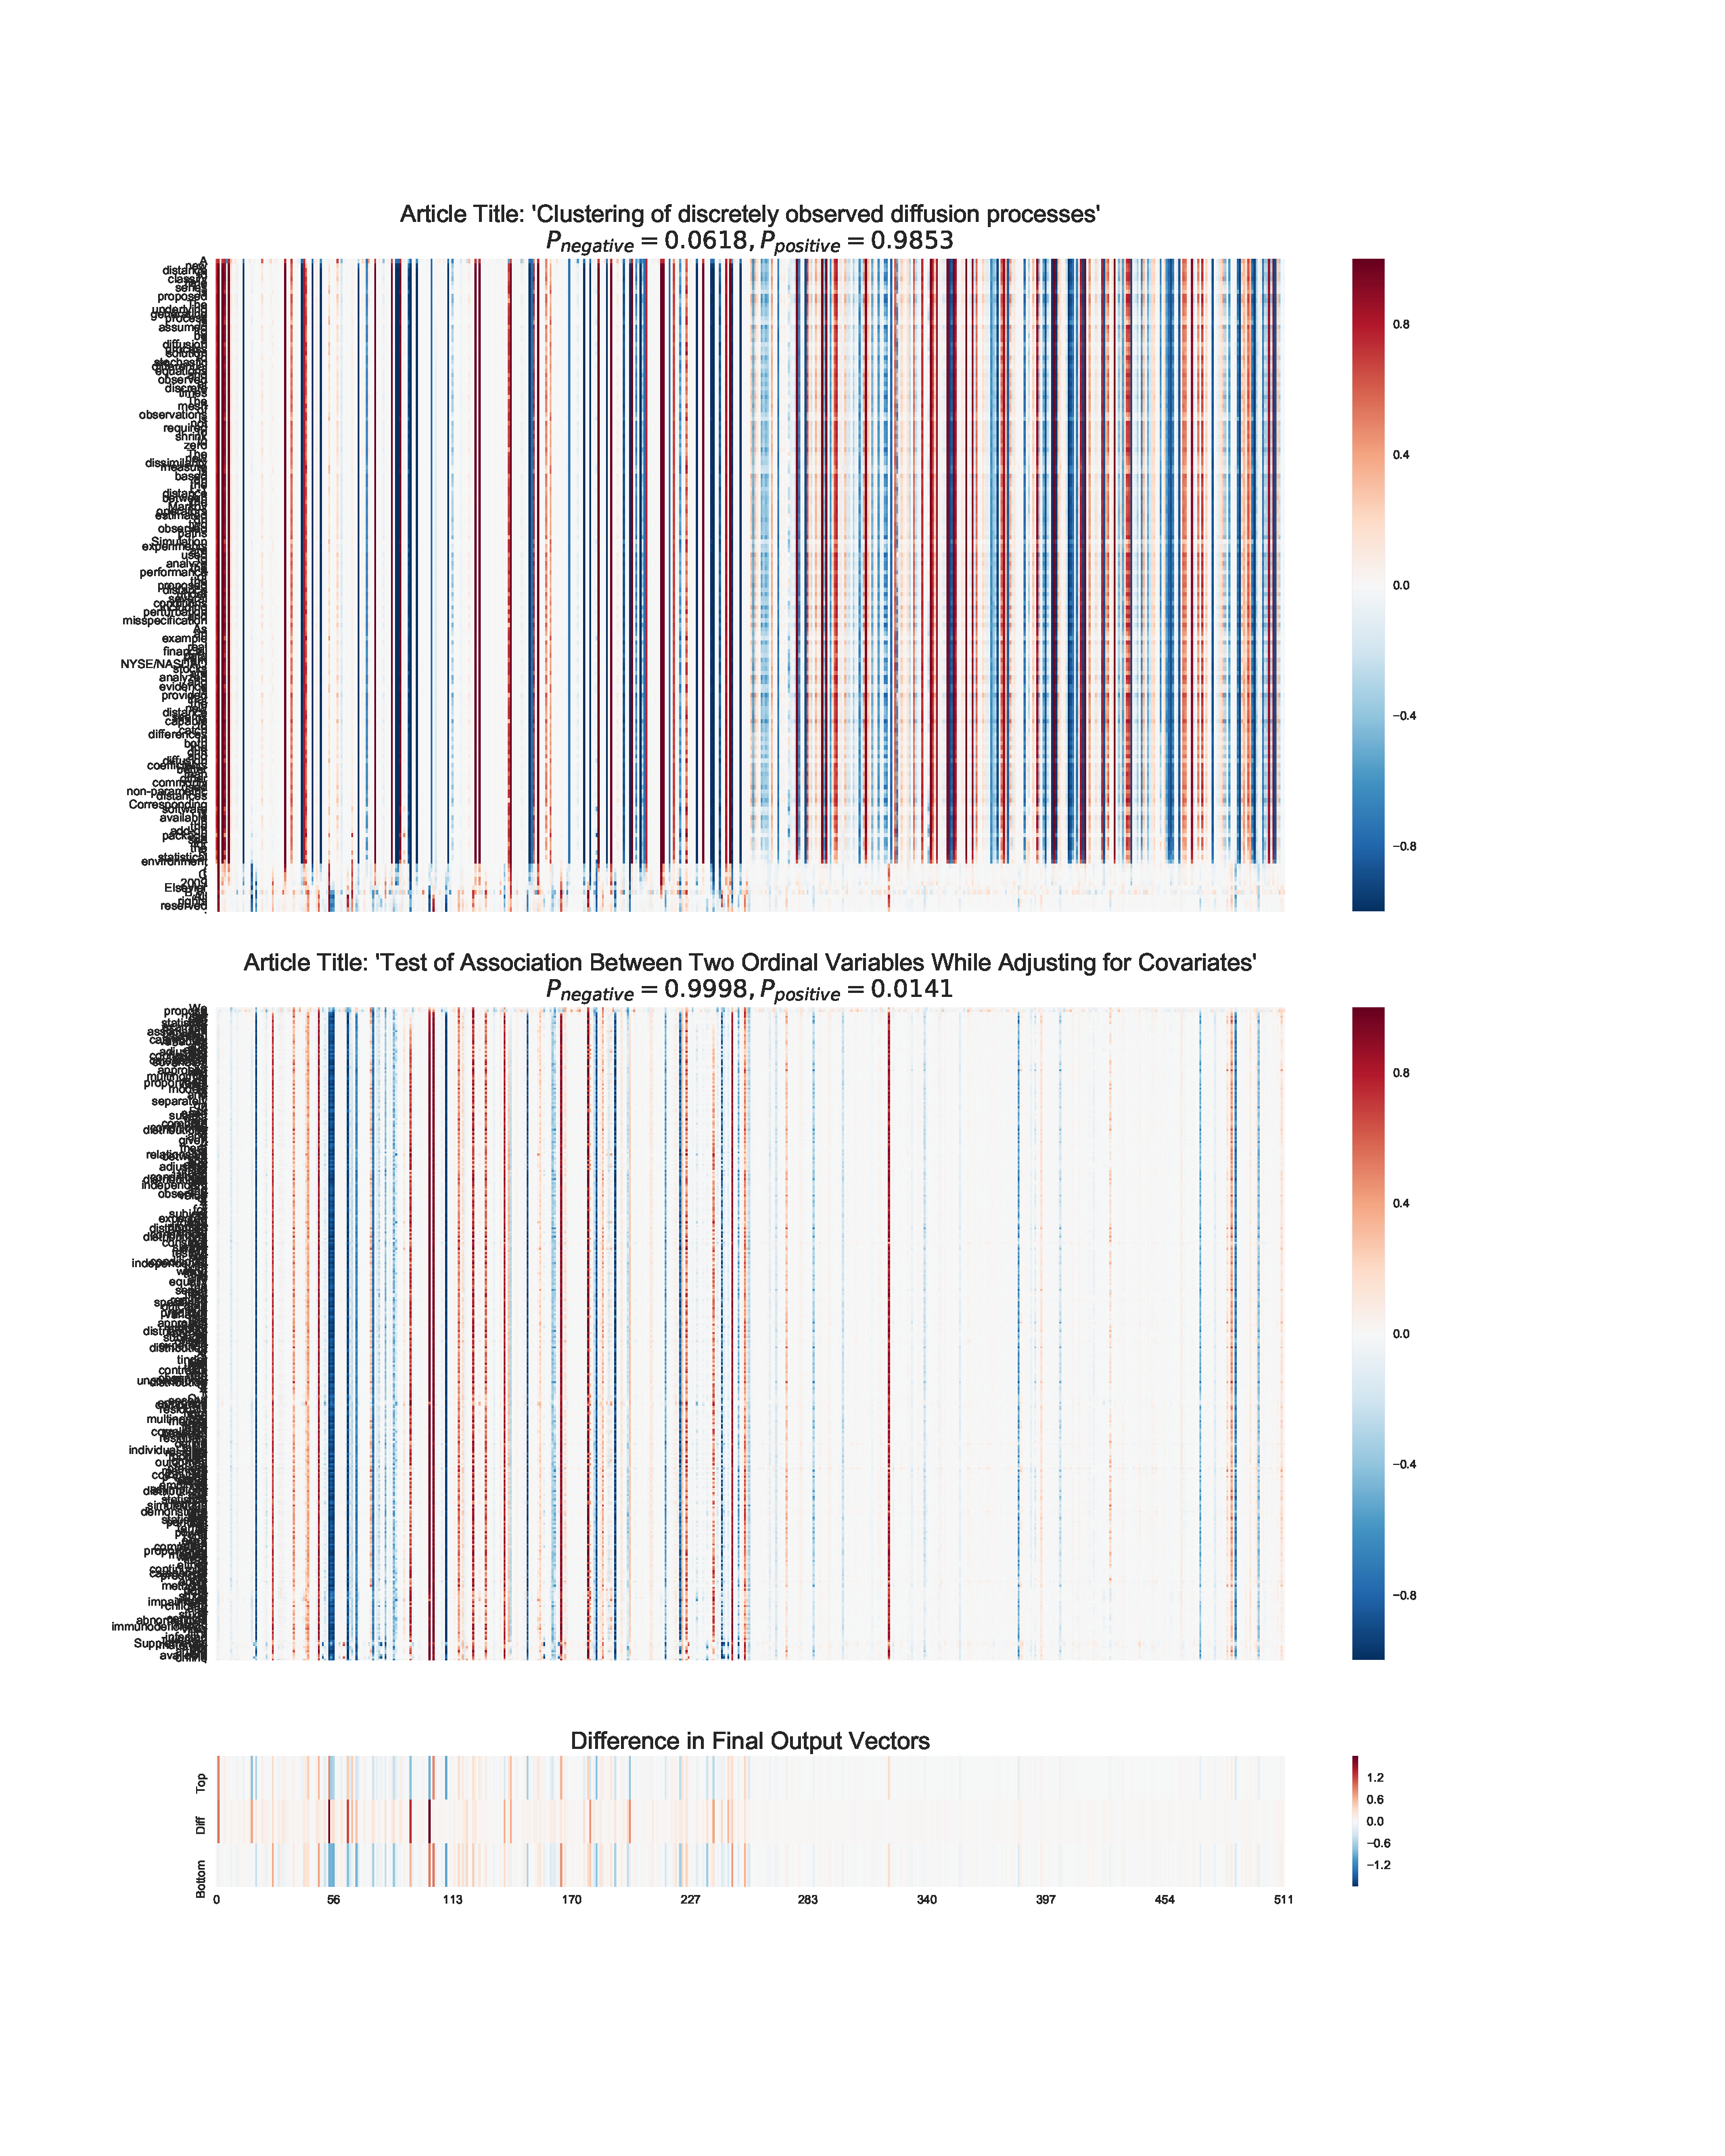
\includegraphics[width=0.55\onecolwid]{comparisonAbstract.pdf}
				\end{adjustbox}
				\caption{RNN activations for each word in two abstracts; the positive example is on top, the negative below it, and a comparison of each input's final output is shown at the bottom.}\label{abstract}
			\end{figure}
		\end{block}
		
	\end{column} 
	
\end{columns}

\end{column} 


\begin{column}{\onecolwid} % The third column
\begin{block}{}
	\begin{table}
		\vspace{2ex}
		\begin{tabular}{|l| cccc|}
			\toprule
			\textbf{Year} & \textbf{\quad  Number of Articles} & \textbf{\quad  Not Software} & \textbf{\quad Software} & \textbf{\quad New Software} \\
			\midrule[2pt]
			2005&	5 235&	4 998&	237&$4.52\%$\\
			2006&	5 806&	5 522&	284&$4.89\%$\\
			2007&	6 255&	5 914&	341&$5.45\%$\\
			2008&	7 085&	6 703&	382	&$5.39\%$\\
			2009&	7 435&	7 047&	388	&$5.21\%$\\
			2010&	7 216&	6 801&	415	&$5.75\%$\\
			2011&	7 767&	7 280&	487	&$6.27\%$\\
			2012&	7 990&	7 519&	471	&$5.89\%$\\
			2013&	8 287&	7 829&	458	&$5.52\%$\\
			2014&	8 336&	7 830&	506	&$6.07\%$\\
			2015&	7 559&	7 095&	464	&$6.13\%$\\
			\midrule[1pt]
			Total & 78 971 &74 538&  4433& $5.61\%$\\
			\bottomrule
		\end{tabular}
		\caption{Per year result across all papers}
	\end{table}
	
\end{block}
\begin{block}{}
	\begin{table}
		\vspace{2ex}
		\begin{tabular}{l cc}
			\toprule
			Highest software count (Training)  &673&	JOURNAL OF STATISTICAL SOFTWARE\\
			& &\\
			Highest software count (Non-training)&171&	\pbox{20cm}{IEEE-ACM TRANSACTIONS ON \\COMPUTATIONAL BIOLOGY\\ AND BIOINFORMATICS}\\
			& &\\
			Highest non-software count (Training) & 1 156 & ANNALS OF STATISTICS\\
			Highest non-software count (Non-training) &3 381& STATISTICS \& PROBABILITY LETTERS\\
			\bottomrule
		\end{tabular}
		\caption{Top journals for each class in training and full dataset}
		\end{table}
	
\begin{figure}
	\includegraphics[width=0.9\linewidth]{countvpub.pdf}
	\caption{Counts for each class against each journal, ordered by number of positive examples, note y axis is log}
\end{figure}

\end{block}

\begin{alertblock}{Discussion}
	\justifying
	As we have shown, the model is capable of identifying complex ideas in textual data. The training set is both relatively small and imperfect; in fact, when the false classifications are examined by an expert, most of them result from errors in the data and not in the model. Thus, by using the model to help generate  cleaner data, a new model could be trained with higher accuracy. The main issue is the false detection rate, which could be reduced by training a cascade of NNs instead of a single one. 
	
	These issues aside, the research undertaken herein demonstrates large-scale detection of new software introduced in scientific literature. The next steps are to do biometric and natural language processing on our corpora as there are many questions we can answer. Of interest to us are `\textit{How programming languages distributed across the sciences?}', `\textit{What properties of new scientific software packages cause them to be accepted by a community?}' and `\textit{What is the relationship between success as an article and success as a software tool?}'.

\end{alertblock}
\begin{alertblock}{Source}
	 The code used for this analysis is available at: \href{https://github.com/reidmcy/New-Software-Identification}{github.com/reidmcy/New-Software-Identification}
\end{alertblock}
\end{column} % End of the third column
%\begin{column}{\sepwid}\end{column} % Empty spacer column
\end{columns}

\end{frame}

\end{document}